\documentclass[conference]{IEEEtran}
\IEEEoverridecommandlockouts
% The preceding line is only needed to identify funding in the first footnote. If that is unneeded, please comment it out.
\usepackage{cite}
\usepackage{amsmath,amssymb,amsfonts}
\usepackage{algorithmic}
\usepackage{graphicx}
\usepackage{textcomp}
\usepackage{xcolor}
\def\BibTeX{{\rm B\kern-.05em{\sc i\kern-.025em b}\kern-.08em
    T\kern-.1667em\lower.7ex\hbox{E}\kern-.125emX}}
\begin{document}

\title{Side Channels for Data Exfiltration from Internet of Things Devices\\
{\footnotesize \textsuperscript{}}
\thanks{}
}

\author{\IEEEauthorblockN{1\textsuperscript{st} Andrew Hughes}
\IEEEauthorblockA{\textit{College of Computer Science} \\
\textit{University of Central Florida}\\
Orlando, Florida \\
andrewhughes@knights.ucf.edu}
\and
\IEEEauthorblockN{2\textsuperscript{rd} Nicholas Omusi}
\IEEEauthorblockA{\textit{College of Computer Science} \\
\textit{University of Central Florida}\\
Orlando, Florida \\
nomusi@knights.ucf.edu}
\and
\IEEEauthorblockN{3\textsuperscript{nd} Zachary Crandall}
\IEEEauthorblockA{\textit{College of Computer Science} \\
\textit{University of Central Florida}\\
Orlando, Florida \\
zcrandall10@knights.ucf.edu}
\and
\IEEEauthorblockN{4\textsuperscript{th} Amro Awad}
\IEEEauthorblockA{\textit{College of Computer Science} \\
\textit{University of Central Florida}\\
Orlando, Florida \\
amro.awad@ucf.edu}
}

\maketitle

\begin{abstract}

Nowadays, processors are being integrated in a wide range of devices, including health care systems, autonomous cars and smart houses. Such devices can be enhanced further by being connected to other devices and interact with users locally and remotely through Internet, which has given a rise to the Internet-of-Things (IoT). In IoT systems, many devices become vulnerable to cyber attacks and being controlled by attackers, such systems include military drones, health systems and mission critical devices. In this paper, we investigate several ways to construct Side channels on IoT devices through  exfiltrating information from air-gapped networks. Such attacks can allow spreading malwares through IoT devices and render forensic operations much harder.

\end{abstract}

\begin{IEEEkeywords}
side channels, internet of things, embedded devices
\end{IEEEkeywords}

\section{Introduction}
As devices are becoming more connected in the modern day, there are new security considerations that must be taken into account. Now when an attacker is able to intrude into a home network it is no longer an attacker just breaching personal computers. Attackers will be able to control cyber-physical connected devices in a consumer's home. 

Covert channel attacks have been identified as one of the major challenges on cyber physical systems. Such attacks allow untraceable communication between attackers, malicious devices and hardware trojans. Moreover, it renders network isolation and solutions to control the spreads of malwares ineffective.


In this paper, we focus on investigating the possibilities of leveraging smart devices behaviours as means for establishing covert channels to communicate with external attackers, especially in air-gapped networks. For instance, we discuss how an attacker can leverage smart bulbs, bluetooth traffic, on-device speakers and HotPlug AVs as methods to construct fast covert channels. 


The rest of the paper is organized as follows. Section \ref{sec:back} discusses the background of the paper. Later, in Section \ref{sec:attacks}, we discuss several ways to construct covert channel and side channel attacks on cyber physical systems. Finally, we conclude our paper in Section \ref{sec:Concl}.

\section{Background}
\label{sec:back}
In this section we explain the problem scenario, and background research detailing means of data exflitration in air-gapped networks. 

%threat model table -- Do we need a table? - true,, they do want us to tuy to say perhaps how an attacker could breach each one of these layers: hardware (factory?), firmware( factory again, update exploit?) s, software (everything in the world), and then networking - I'm going through right now and adding each one of those layers to our channels that we propose

\textbf{Threat Model:} In our paper, we assume a physical attacker who is capable of observing the behavior of different physical systems within the air-gapped network.The attacker does not need to have a full-access to the system, but is sufficient to be able to remotely observe light bulbs, Bluetooth traffic and others. Meanwhile, within the attacked system, a malicious device is trying to communicate a message to the attacker and the external world even though operating on an air-gapped network. The malicious device can be a result of a breach on software, firmware or a hardware trojan.  

Past research has largely looked into side channels and covert channels in servers or personal devices rather than in embedded Internet of Things devices\cite{Opt}\cite{spc}\cite{iOS}. Some have used light sources as effective means to exfiltrate data over air-gaps sources\cite{Opt}. Others mis-use features of complex processors\cite{spc}. 

In this paper we examine a "smart home" environment in which there are many networked Internet of Things devices. We assume that this network of cyber-physical devices is air-gapped from any external network. We assume that an attacker is able to breach these devices, and needs to exfiltrate small amounts of data. Figure 1 shows our scenario, in which many smart devices are connected within a home or small business environment.

\begin{figure}
    \centering
    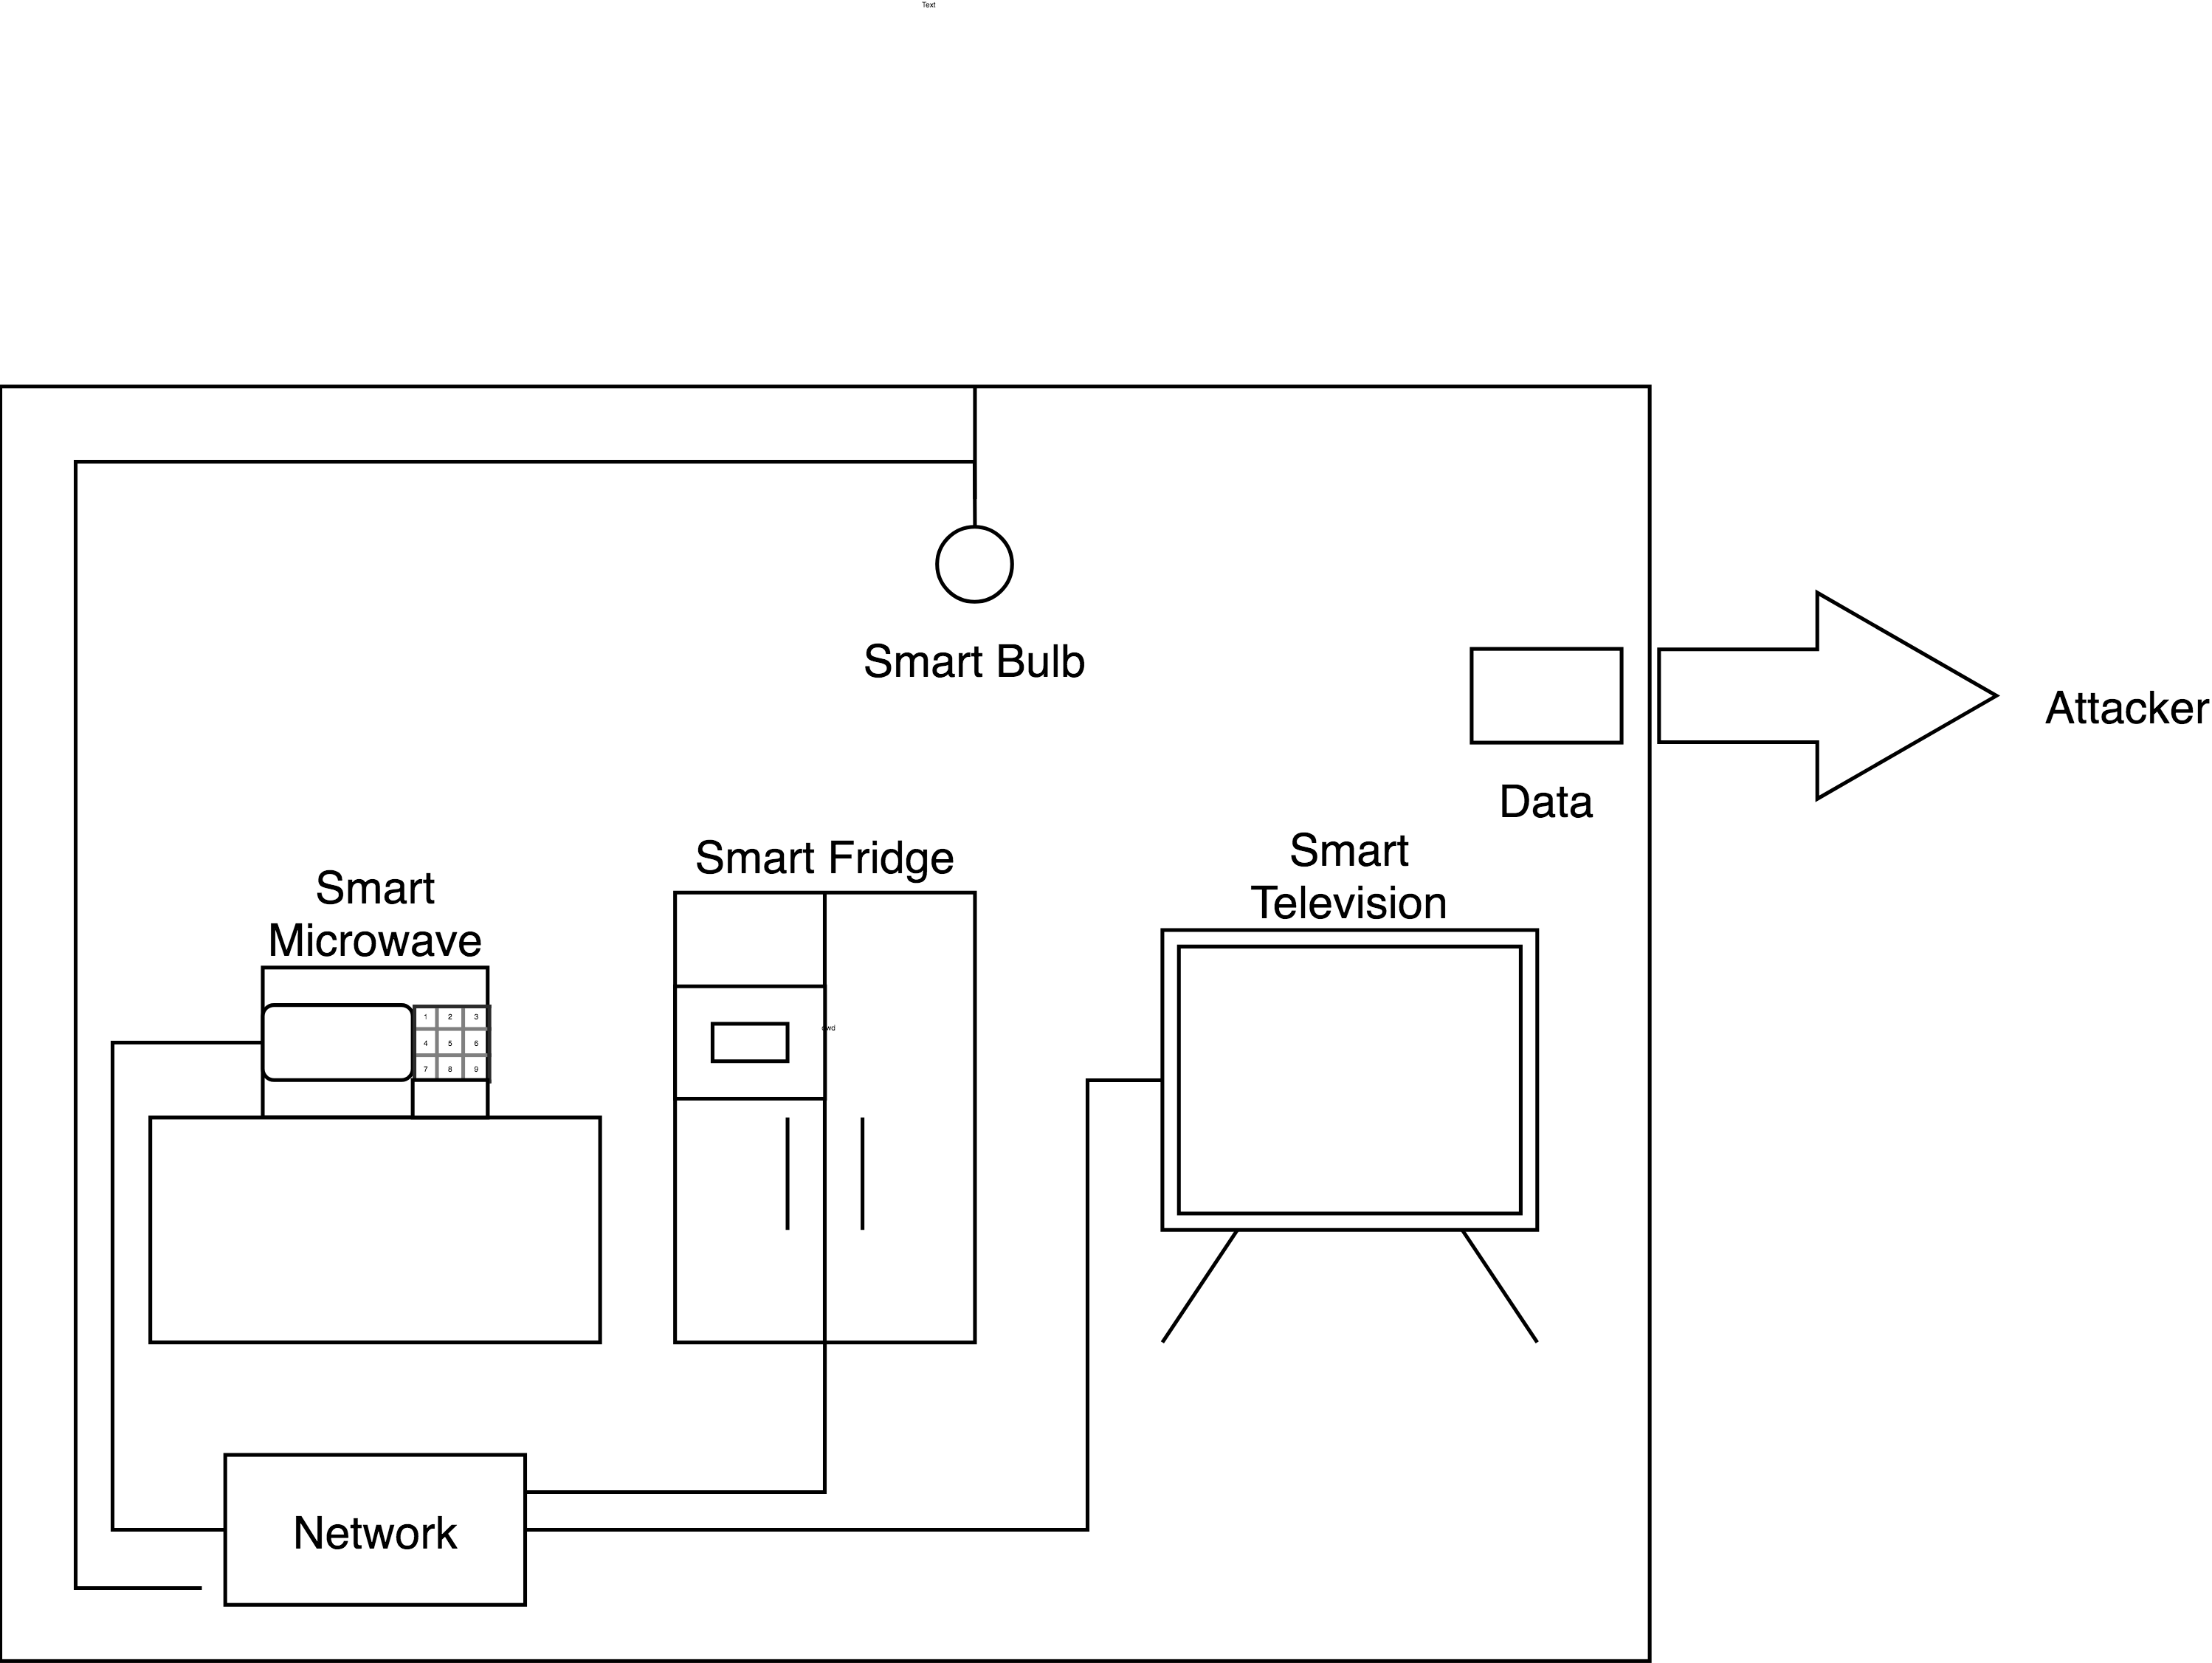
\includegraphics[width=0.5\textwidth]{scenario.png}
    \caption{Proposed "Smart Home" Scenario}
\end{figure}

% talk about layers of smart light bulb

\section{Proposed Side Channels}
\label{sec:attacks}
In this section we discuss channels that can be utilized to exflitrate data according to our scenario. With each channel we discuss possible problems, corrections to those errors, ease of detection, and theoretical bandwidth that can be achieved with each method. In order to exflitrate data, we must send some sort of signal through another means other than the network to which the devices are connected. For our channels, we have a focus on channels present in commodity smart lightbulbs. 

\subsection{Customizable Lighting}

Modern smart light bulbs allow users to customize lighting features to their individual wishes\cite{bt_speaker1}\cite{bt_speaker2}\cite{bt_light1}. Many light bulbs support variable brightness levels, a customizable RGB hue, and often times oscillating patterns which a user can set. This allows many different possible brightness and color combinations that a light can be set to. If an attacker is able to access these settings, this feature can be used to exfiltrate data from the Internet of Things light bulb. Note that an attacker can also rely on light sensors for accurate and fast communication with the malicious device.

We propose two means via which an attacker might be able to control these settings. The first is if the attacker is able to modify firmware on the device. Our second proposal would be if an attacker is able to connect to spoof color change commands to the light bulb.

Once control over these settings is established, an attacker might be able to encode the data which they wish to exfiltrate in differences in light and/or hue. If an attacker chooses to encode data in brightness, they must take into account that this gives them 256 possible values of brightness, and that a person in the vicinity would be able to more easily see differences in brightness. To avoid this we propose that an attacker might be able to cause the light to flicker, or rapidly change brightness, as if the bulb is failing.

An attacker might be able to encode their data in small differences in RGB value differences. A human eye is able to see around 10 million colors\cite{c1}\cite{c2}, and while this is a large amount, the entire RGB spectrum is able to produce \begin{math}256^{3}\end{math}, or approximately 16 million colors. This leaves the possibility that an attacker might be able to use small color differences to transmit their message while not being perceived by a human.

We assume that the attacker would use a camera to receive light data to later decode into data. In both cases it is feasible for an attacker to then receive light information from the room, permitted it is somewhat close to, or has an indirect path to where an attacker is able to view this light. In Figure 2, we show a scenario in which the attacker has direct line-of-sight access to the light, and a scenario in which an attacker has direct line of sight obstructed by something (for example, a door frame), but is still able to receive light that is reflecting off the visible wall in the room. 

This attack could have some shortcomings, mainly in that it will be most effective at night-time where there is little background light. This could restrict the usable times for this side channel. Additionally, if light is indirect, there might be some of the emitted colors mixing with the color of the surface which the light must bounce off of. The receiving device must then calibrate for that, and the differences in broadcasts must then be larger than before, making this potentially more detectable, and lowering the theoretical throughput.

\begin{figure}
  \centering
  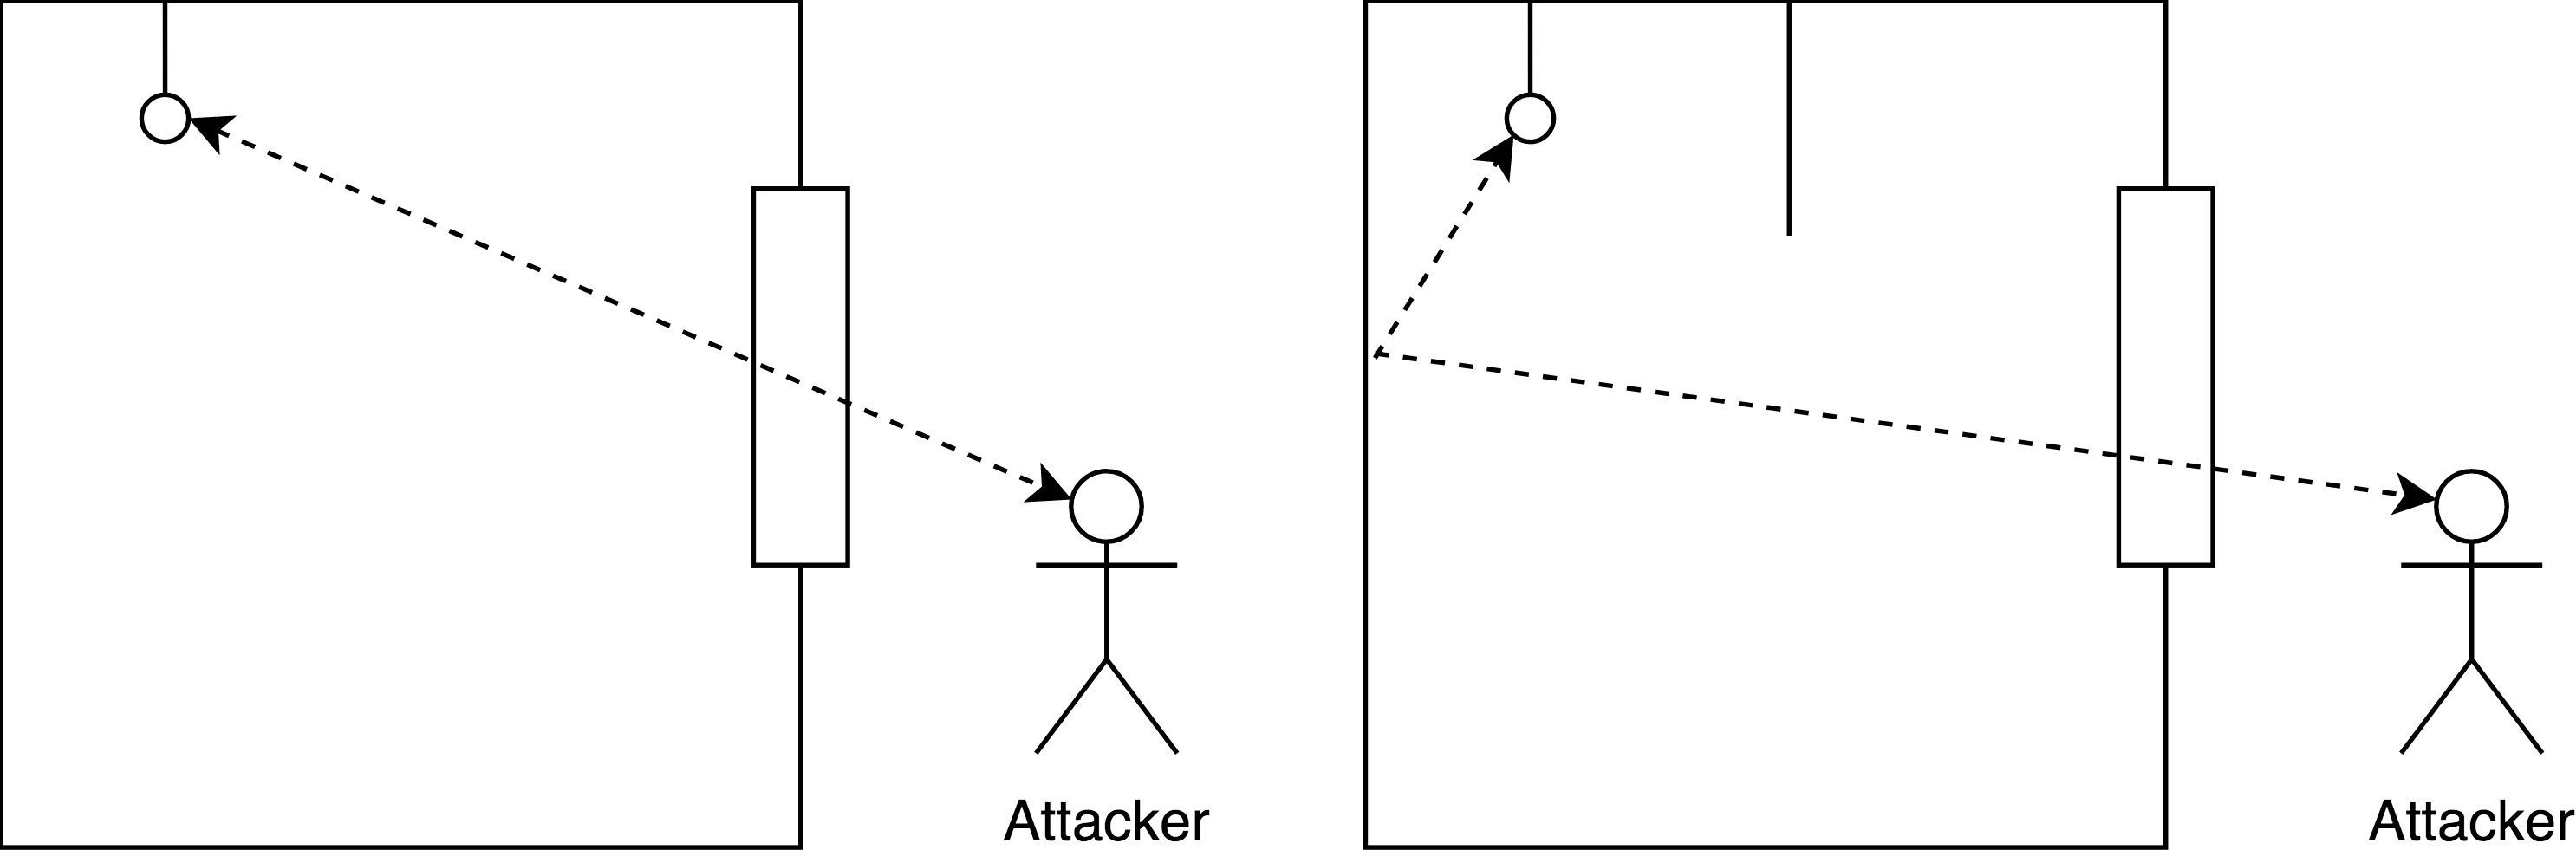
\includegraphics[width=0.5\textwidth]{attacker_lightpaths.png}
  \caption{Paths of light with and without obstruction}
\end{figure}

\subsection{Bluetooth Traffic Analysis}

Many smart light bulbs use Bluetooth to communicate with user devices for control\cite{bt_speaker1}\cite{bt_speaker2}\cite{bt_light1}. We also assume that an attacker is able to generate faulty, or "junk" packets at the firmware and hardware level. This side channel lies upon the ability of an attacker to modulate the frequency at which these "junk" packets are transmitted.

The attacker first translates the message to be exfiltrated into Morse code at the software and firmware level. Then according to the Morse code to be sent, it sends out junk packets, modulating the amount of junk packets. The attacker then has a radio which listens for transmissions on the Bluetooth frequency, and according to the patterns, is able to decode the Morse code and recover the original message.

This attack relies on a relatively quiet Bluetooth radio, and requires some noise cancellation. The signals that must be worked around are other background radios, and legitimate traffic between a controlling phone and the bulb itself. To solve this, we propose a threshold that will be the minimum rate of "junk" packet transfer that will be higher than anticipated background (or legitimate) packet rates. Then an attacker's listener could adjust overall rates to cut out background noise.

As Bluetooth is not something that is enabled on many devices, and many devices will merely discard junk packets, we believe that this approach will be hard to detect, unless someone is actively monitoring the frequency which Bluetooth operates on, which we believe to be unlikely.

\subsection{On Device Speaker}

Some smart light bulbs have integrated speakers intended to play music\cite{bt_speaker1}\cite{bt_speaker2}. It would be possible for an attacker to encode the data which they are exfiltrating into sound at the software level, then transmit this from the hardware level. The attacker would then receive this data via a microphone to next decipher. 

If this approach were taken, a human would easily be able to detect such a system on operation. We then propose that this be used in conjunction with a scheme such as\cite{bd_sound}\cite{co_noodle}, which hide the target data in sound while making it undetectable to humans. 

This side channel would have the shortfall of a receiving sensor needing to be within an audible range so the microphone could decode the data without data loss. It might also have to overcome background noise. In the event of that, we propose an additional threshold scheme such as in B. If this is required, it will likely be much more limited than in the case of Bluetooth, because of a need to raise volumes, which requires more power and may be harder to do on an embedded Internet of Things device.
\subsection{HomePlug AV}

The HomePlug AV standard provides a means for devices to communicate over power lines\cite{homeplug_spec}. In home networks this can create a point to point internet network where the necessary channels for communication already existed, but were not intended for that use. Commercial devices are able to achieve up top gigabit speed. 

\begin{figure}
  \centering
  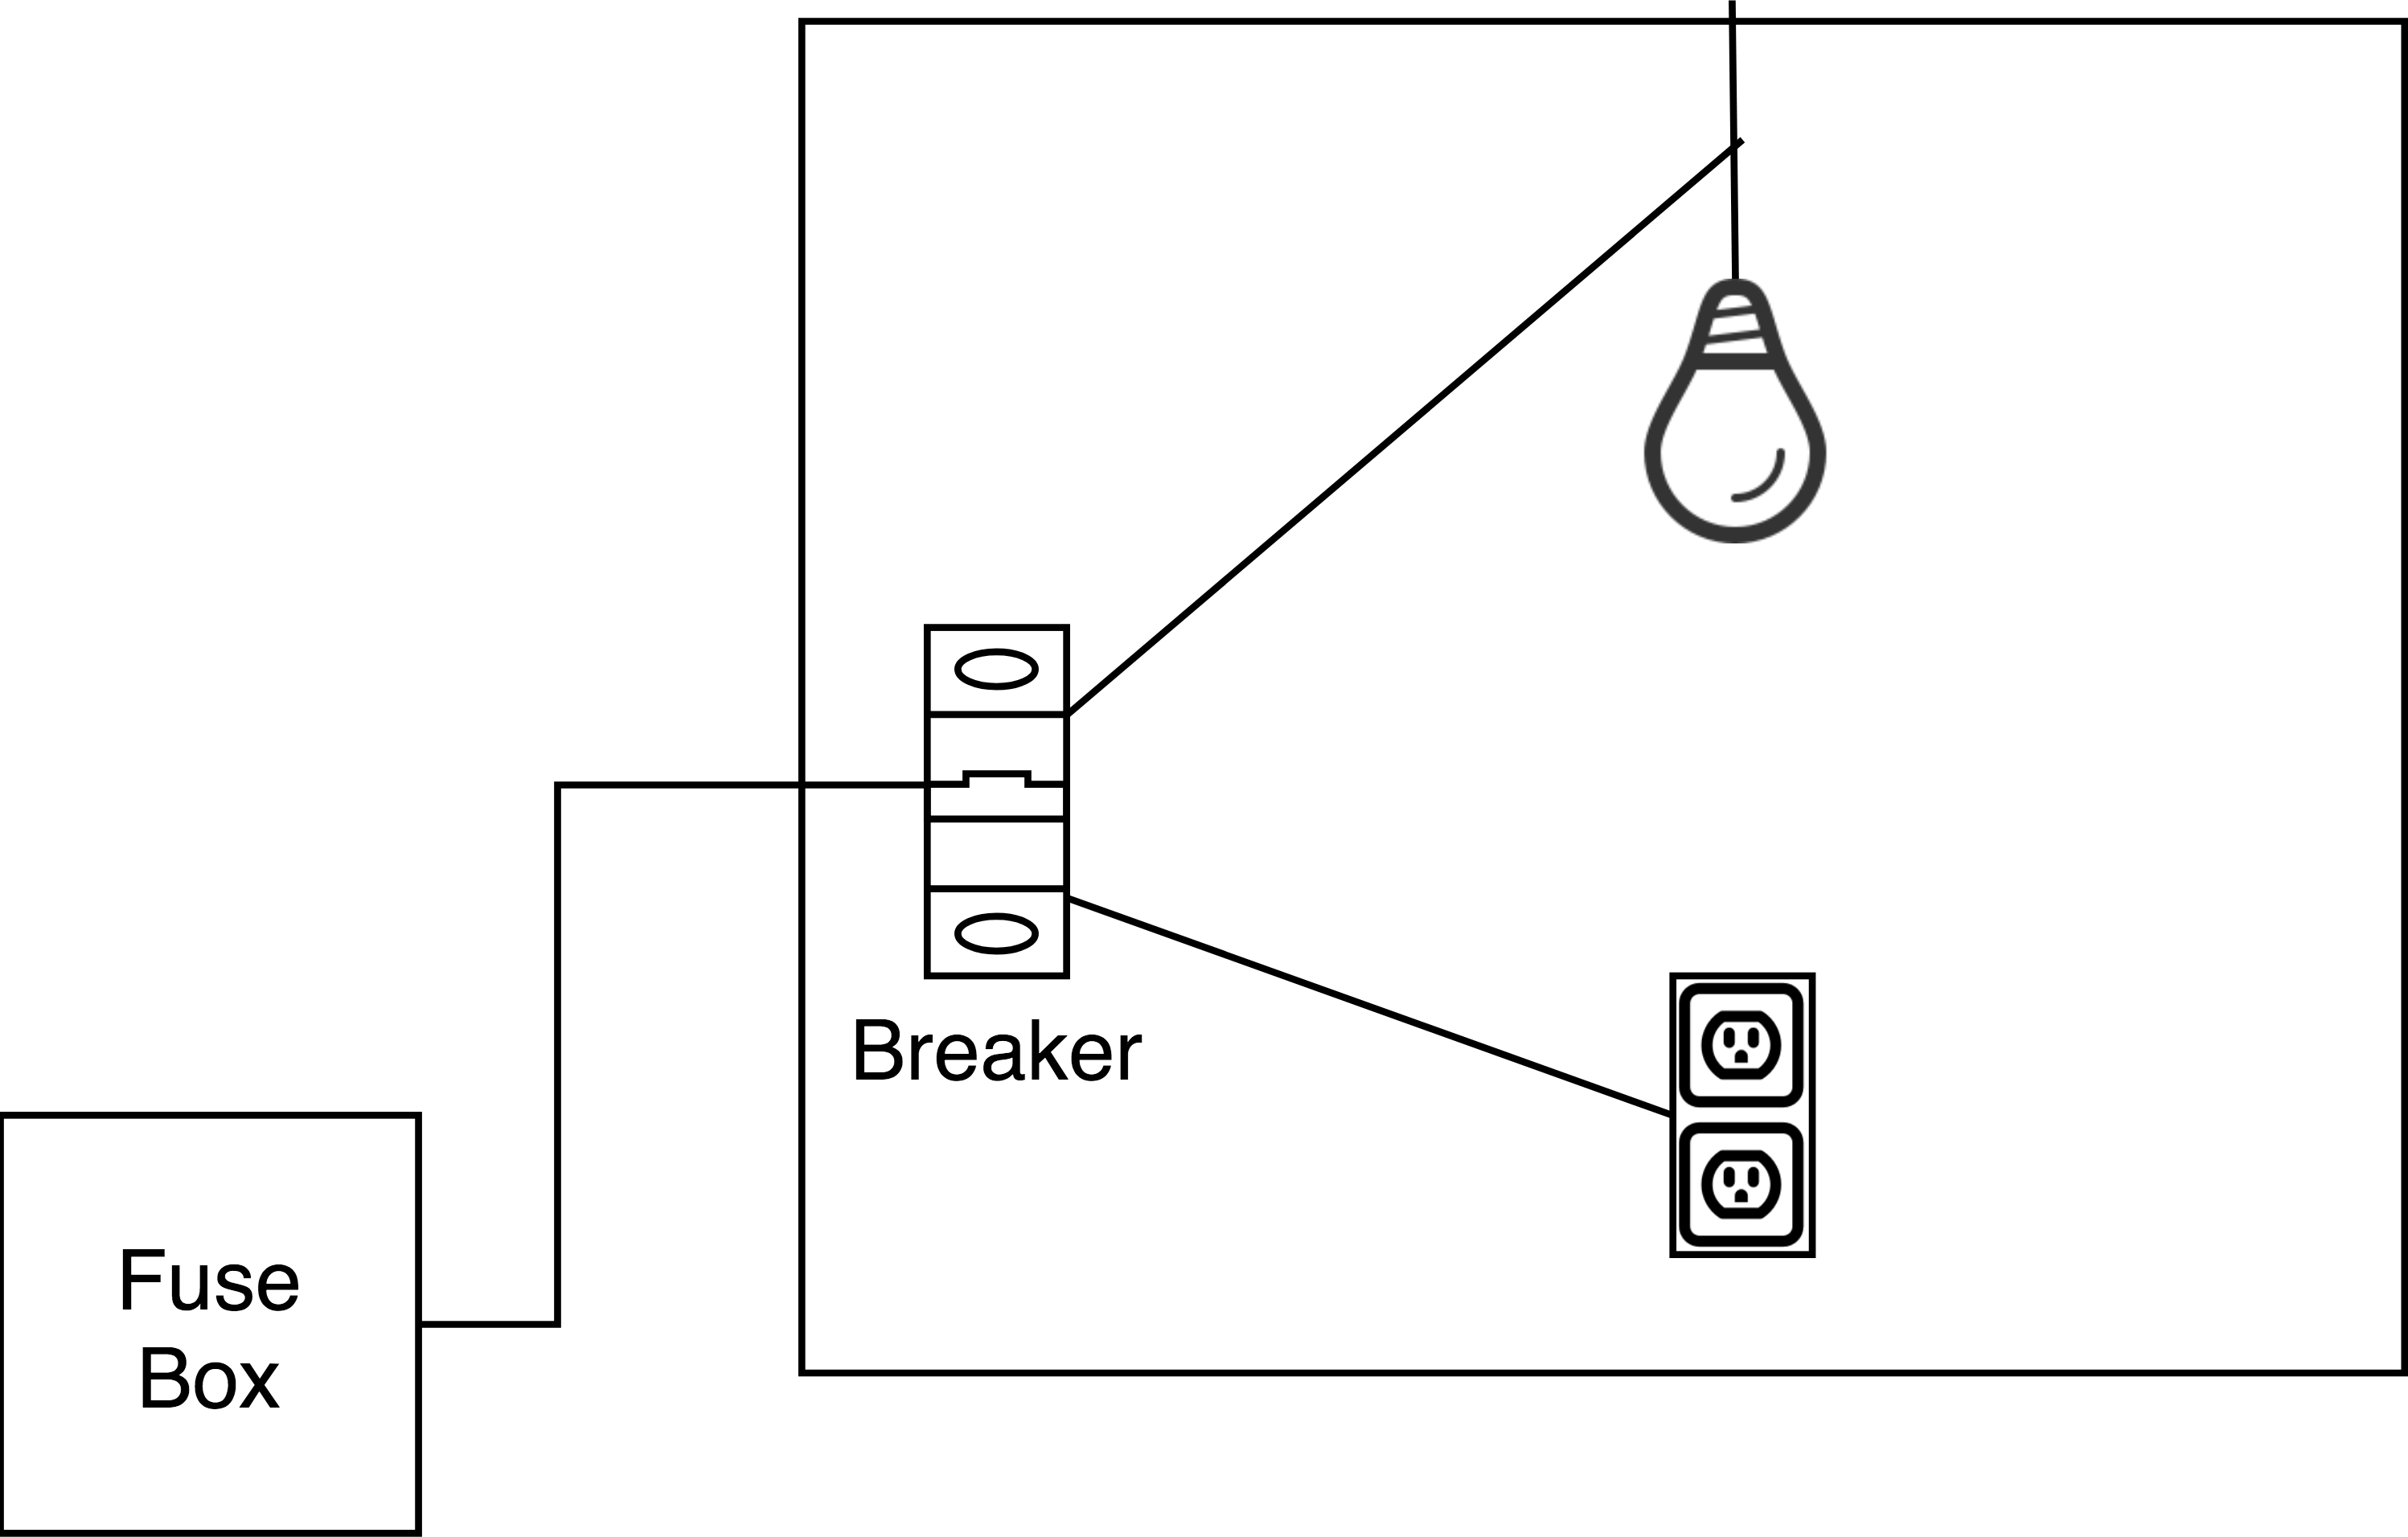
\includegraphics[width=0.5\textwidth]{connection.png}
  \caption{Diagram showing light bulb and outlet on same circuit}
\end{figure}

HomePlug AV is promising because the receptacle a light bulb is inserted into is often on the same breaker as the rest of an electrical system in a house or business, and on the same lines. We believe that it is fair to assume that an attacker might be able to connect their receiving device to an outlet, and thus have a gigabit-speed link to exfiltrate data from the light bulb. 

\subsection{System Management Interrupts}
As stated in proposal A, many modern smart light bulbs are able to have a "rainbow" mode, or "party" mode. In this setting the colors of light bulbs alternate along a pre-set spectrum and timing.

We propose that if an attacker is able to alter the firmware of the devices, they could possibly use processor-heavy methods to cause the integrated circuit to trigger a System Management Interrupt (SMI) in the hardware, in which execution is halted until the integrated circuit has cooled. In this case, an attacker could encode data in system management interrupts. While viewing the color oscillations, an attacker could then note when the transitions hang, and recover the message.

The data would be encoded in a fashion similar to B, in Morse code, with the rate being synchronized to a receiving camera sensor's frames per second.  Upon a color hang, the frame count that the oscillation is then noted and stored. Meanwhile this data will be deciphered into the data being exfiltrated.

The likely-hood of such a "rainbow" or "party" mode being used in a sensitive environment is unlikely, though it could be triggered in firmware when there is little activity around the device, and it is presume that there is no person present to detect this. Another pitfall is that it might be harder to detect (like in A), during the daytime when the differences in light would be harder to detect.

\subsection{Possible Enhancements to Proposed Side Channels}
An attacker can both improve the message transfer rate and improve correctness by utilizing compression and check-sums. For these, we assume that the data that is being exfiltrated is a small amount of ASCII text. If that is not the case then other compression schemes other than those noted here may be more effective for reducing the total data an attacker needs to transmit.
\begin{figure}
    \centering
    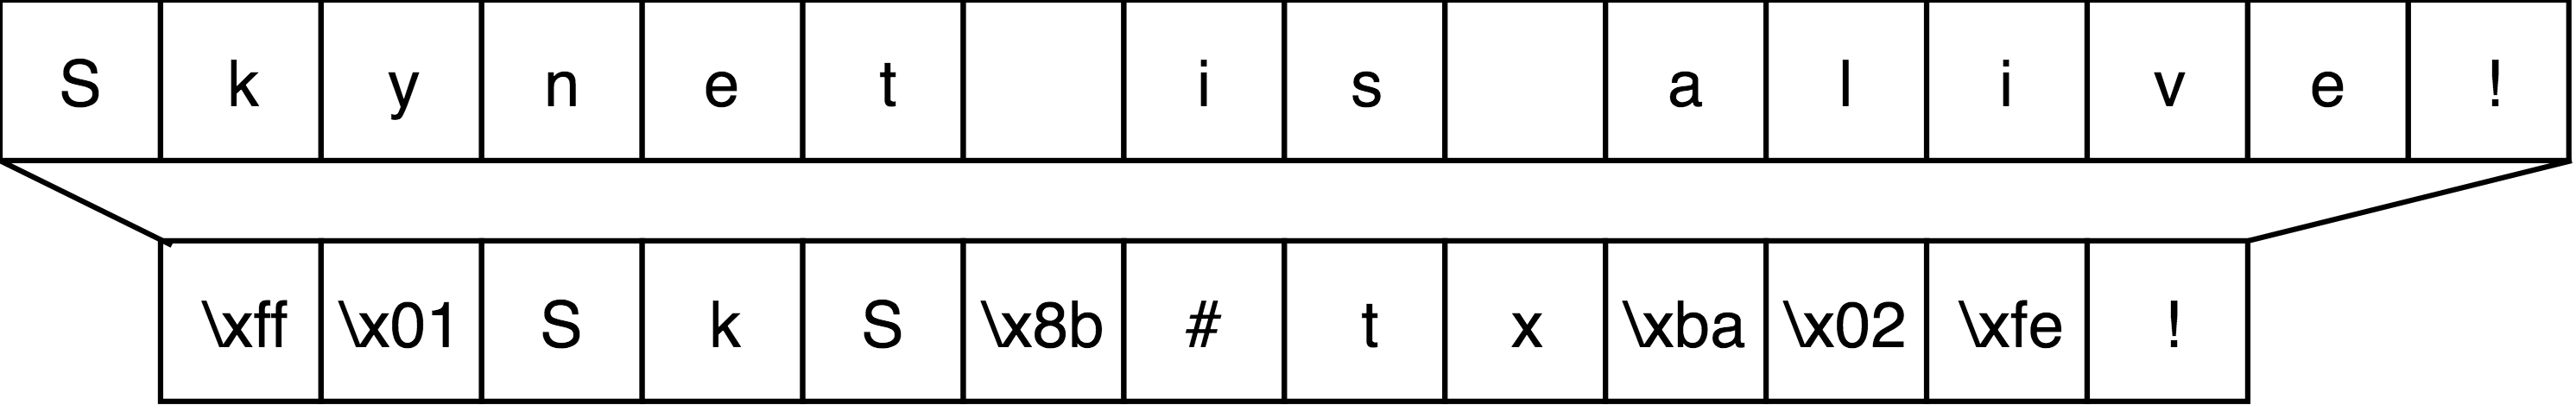
\includegraphics[width=0.5\textwidth]{text_compression_smaz.png}
    \caption{Example string before and after compression}
\end{figure}

If an attacker's data that they wish to exfiltrate is largely ASCII data, for example: ``Skynet is alive!'', then they might be able to use compression algorithms that cater towards small ASCII strings, such as smaz\cite{smaz}. With our example string, which is 16 characters long, we were able to reduce the size that would need to be transmitted to 13 bytes after compression with smaz. Other compression schemes that cater to the data sent could be applied. For example, if the payload is often ASCII English, then an attacker could use a dictionary to avoid transmitting full words.

Simple check-sums that are appended to transmitted messages before any compression is done can help ensure that the messages received are correct, or allow for the receiving devices and sensors to be better calibrated for the environment in which deployment happens. These could be as simple as modular sums of characters to make sure the right ASCII message has been received, and if there is a mismatch the message can be received again.

\section{Conclusion}
\label{sec:Concl}

In this section we conclude our proposed attacks, and compare them. Our first approach relies on encoding data through the color of the light bulb, which can be observed and received by an external attacker or maybe a sensor. Later, we discuss how a device speaker can be utilized for the same purpose. We also discuss how Bluetooth signals be also used to construct covert channels. Finally, we discussed how the HomePlug AV and System Management Interrupts can be leverage for establishing covert channels as well. In summary, we observe that there are several means to construct covert channels in air-gapped networks that use smart bulbs.
%In table X, we state all of our attacks, the layers they rely on, how easily detected they are, and their bandwidth. Overall, we believe that X will be the best approach overall, because of y, in the case of z. Otherwise ....

\begin{thebibliography}{00}
\bibitem{c1} Calkins, D., ``Mapping color perception to a phsiological substrate''. in \textit{The Visual Neurosciences Volume 1},  2004., p. 989-1002,

\bibitem{c2} Wyszecki, G. and Judd, D. ``Color in Business, Science and Industry''. New York: John Wiley \& Sons, Ltd., 1975 p.388.

\bibitem{bd_sound} N. Roy, H. Hassanieh, and R. R. Choudhury.  ``Backdoor: Making Microphones Hear Inaudible Sounds''. In \textit{Proceedings of the 15th Annual International Conference on Mobile Systems, Applications, and Services (MobiSys)}, pp. 2-14, New York, NY, June 2017.

\bibitem{co_noodle} T. Vaidya, Y. Zhang, M. Sherr, and C. Shields. ``Cocaine noodles: exploiting the gap between human and machine speech recognition''. In \textit{USENIX Workshop on Offensive Technologies(WOOT)}, Washington, D.C., Aug. 2015.

\bibitem{smaz} S. Sanfilippo. ``SMAZ - compression for very small strings''. Github, Feb. 2012. https://github.com/antirez/smaz
% next citation is a bit odd, need to have Dr. Awad check
\bibitem{homeplug_spec} Alliance, HomePlug Powerline ``Homeplug AV White Paper''. HomePLug Power Alliance, Inc, 2005

\bibitem{bt_speaker1} Amazon.com ``RAYWAY Led Bluetooth Bulb''. Amazon.com, 2018. https://www.amazon.com/RAYWAY-Bluetooth-Controlled-Dimmable-Multicolored/dp/B072KH45L6

\bibitem{bt_speaker2} Amazon.com ``Texsens LED Light Bulb''. Amazon.com, 2018 https://www.amazon.com/Texsens-Bluetooth-Speaker-Changing-Wireless/dp/B01CP1QB72

\bibitem{bt_light1} Amazon.com ``Magic Bluetooth Bulb''. Amazon.com, 2018. https://www.amazon.com/gp/product/B0176HB8C8

\bibitem{Opt} M. Guri, O Hasson, G. Kedma, and Y.Elovic. ``An Optical Covert-Channel to leak Data through an Air-Gap''. In \textit{ArXiv E-prints}, arXiv:1607.03946. Jul. 2016.

\bibitem{iOS} C. D'Orazio, K. Choo, and L. Yang. ``Data Exfiltration From Internet of Things Devices: iOS Devices as Case Studies''. In \textit{IEEE Internet Of Things Journal}, vol. 4, pp. 524-535 Apr. 2017.

\bibitem{spc} P. Kocher, D. Genkin, D. Grus, Et. al. ``Spectre Attacks: Exploiting Speculative Execution''. In \textit{ArXiv E-prints}, arXiv:1801.01203. 2018

\end{thebibliography}
\vspace{12pt}
\end{document}
